%%% Fiktivní kapitola s instrukcemi k PDF/A

\chapter{Experimenty a výsledky}

V této kapitole se podíváme na tři typy experimentů, které s naším systémem
můžeme provádět. Knihovna implementuje několik různých přístupů jak roboty
řídit a jak je vyvíjet pomocí evolučních algoritmů. Následující experimenty
předvedou vzorek z těchto přístupů. 

Cílem všech následujících experimentů je pomocí evolučních algoritmů vyvinout
zvoleného robota tak, aby byl schopný stabilního pohybu v simulovaném prostředí
v předem určeném směru. Kvalita jedinců je pak jednoduše vypočtena dle
následující rovnice:

\begin{equation} \label{fitness_calc}
    fitness = x - 0.5\cdot|y|
\end{equation}

Každý jedinec začíná svůj simulační běh v prostředí v počátku na souřadnicích
$(x,y) = (0,0)$, tedy v rovnici \label{fitness_calc} jsou $x$ a $y$ vzdálenosti
od počátku, které jedinec v simulovaném prostředí urazil (buď do vypršení
limitovaného času na simulaci, nebo do dosažení podmínky předčasně ukončující
simulační běh -- např. pád robota).

V prvním experimentu v sekci \ref{exp1} se podíváme na ověření, zda pro řízení
jednoduchých robotů nám stačí základní evoluční algoritmy a pro složitější
roboty (s větším množstvím stupňů volnost) potřebujeme pokročilé přístupy.
V následujících dvou experimentech v sekci \ref{exp2} popíšeme experimenty
předvádějící možnost evolučního vývoje jak řízení tak morfologie robotů.

\section{Vývoj řízení robotů} \label{exp1}

V této sekci se zaměříme na vývoj řízení robotů. Vývoj řízení je ovlivněn
hlavně zvoleným řídícím agentem, který popisuje zvolený evoluční algoritmus.
Tento agent z genetických informací kóduje vstupy pro motory (nastavení kloubů)
robota. Určití agenti mohou využívat přímou reprezentaci vstupů pro motory, kde
sama genetická informace reprezentuje nastavení motorů. Jiní využívají nepřímou
reprezentaci, kde genetické informace slouží jako parametry pro generování
aktuálního nastavení motorů.

\begin{figure}[!htb]
    \centering
    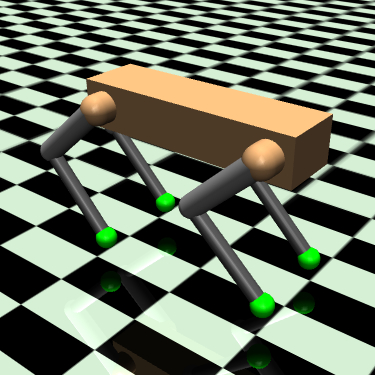
\includegraphics[width=0.4\textwidth]{../img/crop_SpotLike.jpg}
    \caption{Robot \emph{SpotLike}}
    \label{fig:robot:spotlike}
\end{figure}

%TODO: imp ref robots SPOT
První pokus se bude snažit vyvinout řízení pro pokročilého robota v projektu
označovaném jako \emph{SpotLike} (blíže popsaný v implementaci v sekci
\ref{robot:Spot}). Jedná se o robota kráčejícího na čtyřech nohách, kde každá
noha má 3 stupně volnost (tedy 12 celkem pro celého robota). Můžeme ho tedy
řadit mezi roboty, u kterých již bude obtížnější vyvinout stabilní pohyb v
určeném směru.

Kráčení, kterého bychom u robotů chtěli dosáhnout, si můžeme představit jako
poměrně jednoduchý periodický pohyb. Proto se pro vývoj řízení pokusíme využít
agenty, kteří interně podle parametrů generují periodické hodnoty pro motory
robotů. 

Nejdříve se pokusíme řízení robota vyvinout pomocí evolučního
algoritmu, který kóduje nastavení motorů pomocí základních periodických funkcí
(agent popisující tento algoritmus popsán v implementaci v sekci
\ref{agent:sinefull}). Každý motor robota má v tomto případě přiřazenou vlastní
periodickou funkci a genotyp jedinců specifikuje parametry těchto periodických
funkcí (4 parametry pro každý kloub -- amplituda, frekvence, $x$ a $y$ posun).

Evoluční algoritmus poběží \textbf{200 generací} se \textbf{100} náhodně
inicializovanými jedinci. Pro vyhodnocení bude celý běh evolučního algoritmu
bude \textbf{pětkrát opakován} vždy s novou náhodně vygenerovanou první populací.

% TODO: graph resolution

\begin{figure}[!h]
    \centering
    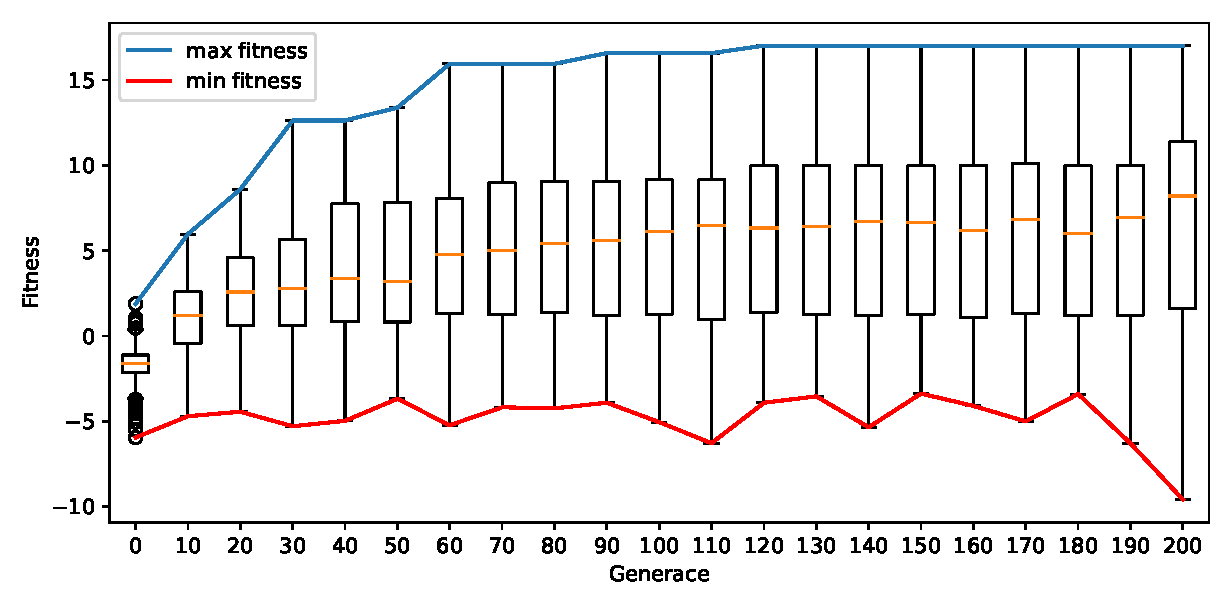
\includegraphics[width=1\textwidth]{../img/experiment1_Sine_10ticks.pdf}
    \caption{Průběh fitness populace v experimentu se základním agentem}
    \label{exp:first_sinefull}
\end{figure}

Graf na obrázku \ref{exp:first_sinefull} vizualizuje průběh vývoje fitness
hodnot za běhu výše popsaného evolučního algoritmu. Data jsou vytvořena
kombinací záznamů o fitness hodnotách v dané generaci ze všech pěti nezávislých
běhů.

Z grafu se ukazuje, že tento přístup vývoje řízení dosáhl maximální hodnotu
fitness okolo 10 a absolutní většina populace není schopna většího posunu. 

Pro porovnání volíme pokročilého agenta, kódujícího nastavení motorů pomocí
omezených Fourierových řad (agent popsán v sekci \ref{agent:TFS}). Tento agent
je na úkor malého zvětšení genotypu, oproti předchozímu agentovi schopný
generovat mnohem komplexnější periodické funkce popsané skládáním několika
funkcí sinus.

Stejně jako v předchozím běhu, algoritmus poběží 200 generací se 100 jedinci a
bude opět pětkrát zopakován.

\begin{figure}[!h]
    \centering
    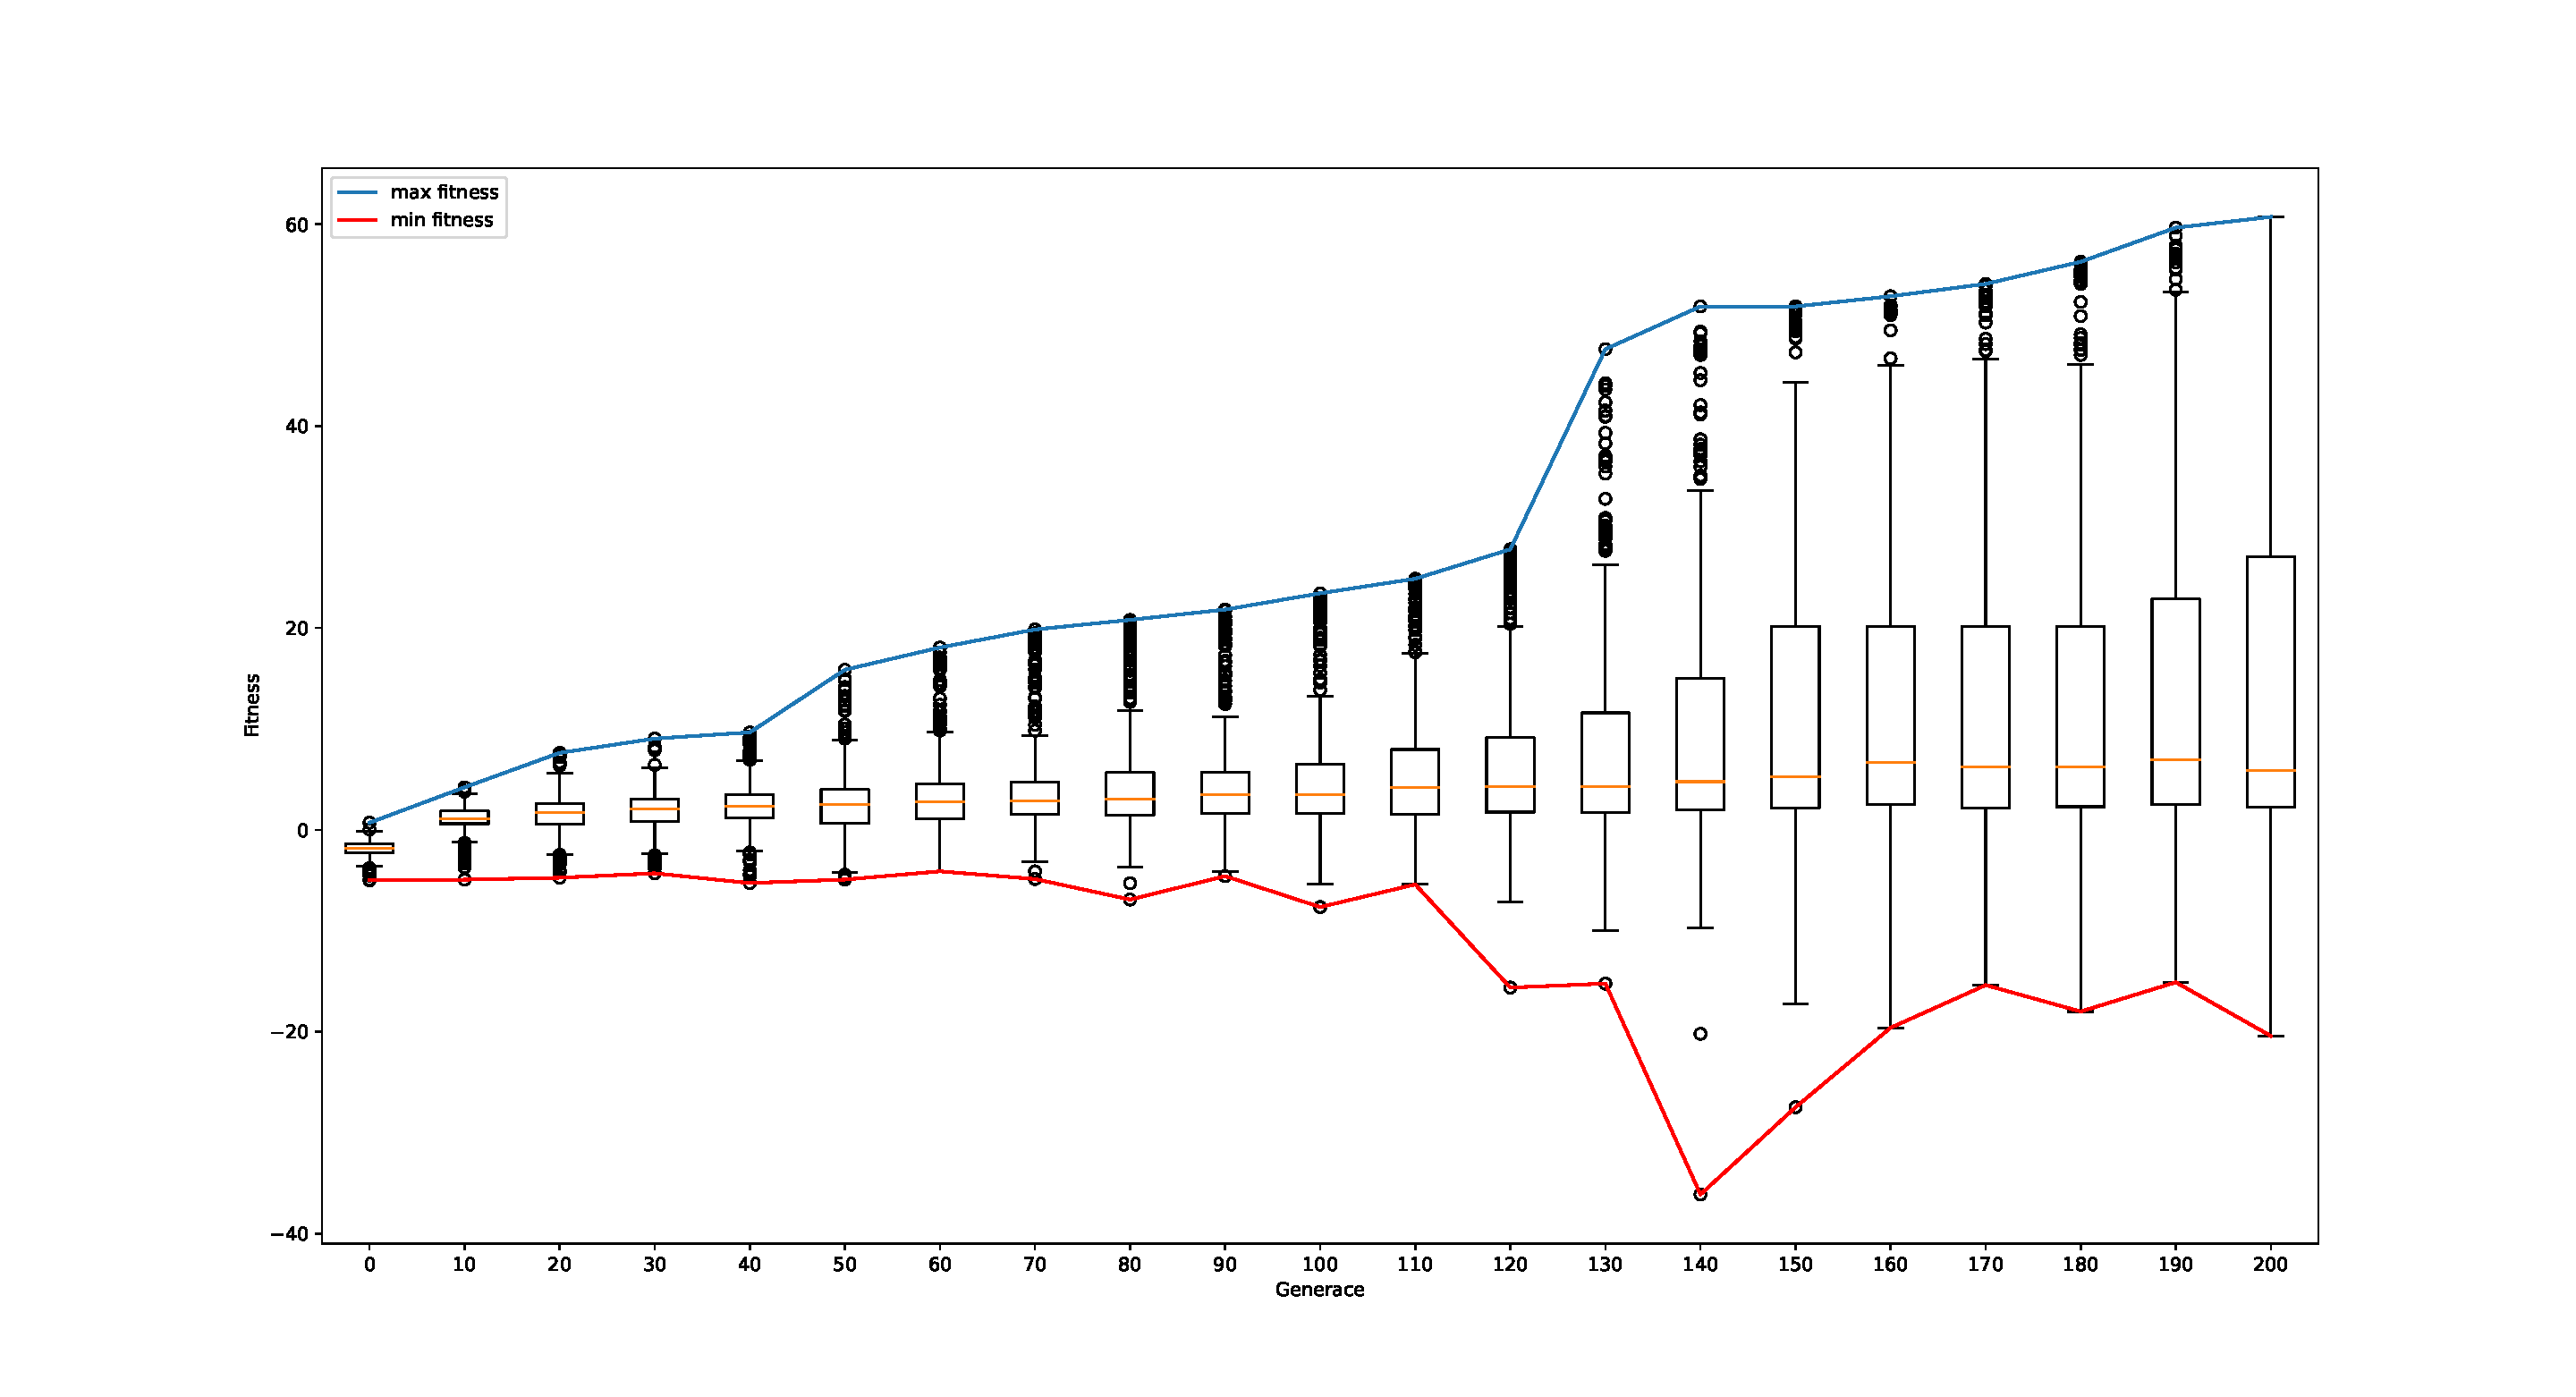
\includegraphics[width=1\textwidth]{../img/experiment1_TFS_10ticks.pdf}
    \caption{Průběh fitness populace v experimentu s pokročilým agentem}
    \label{exp:first_TFS}
\end{figure}

Graf \ref{exp:first_TFS} průběhu vývoje fitness hodnot z experimentu s
pokročilým agentem ukazuje, že tento agent již je schopný vyvinout stabilní
pohyb i pro zadaného komplexního robota. Maximální fitness hodnota, které při
vývoji agent dosáhl se pohybovala okolo 60. Zároveň poměrně velká část populace
byla schopná dosáhnout výsledků, přesahující nejlepší výsledky jednoduššího
agenta. Průběh vývoje dále naznačuje, že pokud bychom navýšili počet generací,
tak by byla možnost pohyb dále optimalizovat a dosáhnout tak ještě vyšší
fitness. 

Z experimentu, vedle hodnot pro zpětné statistické zpracování dat, dostaneme i
nejlepšího jedince, který byl otestován v poslední generaci běhu evolučního
algoritmu. Jelikož naše simulované fyzikální prostředí je deterministické,
máme možnost jedince nahrát zpět do simulace a vizualizovat tak nejlepší řešení
daného evolučního algoritmu. 

Ruční kontrolou těchto výsledků jsme dále zjistili, že pouze část (dva z pěti
běhů) dosáhly takového pohybu, který bychom od robota této morfologie
očekávali. Pohybovali se tedy až na menší odchylku rovně, způsobem
připomínající chůzi skutečných čtyřnohých zvířat. Zbylé běhy vyvinuly pohyb,
který sice je schopný stabilní, ale ne zcela estetické chůze. Roboti se v
těchto případech posouvali bokem vpřed, využívající většího rozsahu v rotaci
(\emph{kyčelních}) kloubů pro stabilizaci.

Osobně si myslím, že vývoj estetického pohybu pro tohoto robota je možný jen s
malou úpravou hodnotící, která by například penalizovala rotaci těla od
požadovaného směru pohybu. Myslím si, že chůze stranou je kvůli rozsahu
(\emph{kyčelních}) kloubů hlavně v ose délky těla robota, mnohem snazší na
dosažení, tvořící zde silné lokální optimum. Agenti totiž velmi rychle
konvergují ke způsobům chůze, které jsou stabilní a chůze stranou je oproti
vratké chůzi rovně mnohem stabilnější. Úprava hodnotící funkce by měla
být schopna toto lokální optimum penalizovat.

\section{Vývoj řízení a morfologie robotů} \label{exp2}
\subsection{Oddělený vývoj řízení a morfologie}
\subsection{Simultánní vývoj řízení a morfologie}

\section{Diskuze výsledků}
